\documentclass[a4paper, 12pt, twoside]{article}


%------------------------------------------------------------------------
%
% Author                :   Lasercata
% Last modification     :   2022.02.26
%
%------------------------------------------------------------------------


%------ini
\usepackage[utf8]{inputenc}
\usepackage[T1]{fontenc}
\usepackage[french]{babel}
%\usepackage[english]{babel}


%------geometry
\usepackage[textheight=700pt, textwidth=500pt]{geometry}


%------color
\usepackage{xcolor}
\definecolor{ff4500}{HTML}{ff4500}
\definecolor{00f}{HTML}{0000ff}
\definecolor{0ff}{HTML}{00ffff}
\definecolor{656565}{HTML}{656565}

\renewcommand{\emph}{\textcolor{ff4500}}
\renewcommand{\em}{\color{ff4500}}

\newcommand{\strong}[1]{\textcolor{ff4500}{\bf #1}}
\newcommand{\st}{\color{ff4500}\bf}


%------Code highlighting
\usepackage{listings}

\definecolor{cbg}{HTML}{272822}
\definecolor{cfg}{HTML}{ececec}
\definecolor{ccomment}{HTML}{686c58}
\definecolor{ckw}{HTML}{f92672}
\definecolor{cstring}{HTML}{e6db72}
\definecolor{cstringlight}{HTML}{98980f}
\definecolor{lightwhite}{HTML}{fafafa}

\lstdefinestyle{DarkCodeStyle}{
    backgroundcolor=\color{cbg},
    commentstyle=\itshape\color{ccomment},
    keywordstyle=\color{ckw},
    numberstyle=\tiny\color{cbg},
    stringstyle=\color{cstring},
    basicstyle=\ttfamily\footnotesize\color{cfg},
    breakatwhitespace=false,
    breaklines=true,
    captionpos=b,
    keepspaces=true,
    numbers=left,
    numbersep=5pt,
    showspaces=false,
    showstringspaces=false,
    showtabs=false,
    tabsize=4,
    xleftmargin=\leftskip
}

\lstdefinestyle{LightCodeStyle}{
    backgroundcolor=\color{lightwhite},
    commentstyle=\itshape\color{ccomment},
    keywordstyle=\color{ckw},
    numberstyle=\tiny\color{cbg},
    stringstyle=\color{cstringlight},
    basicstyle=\ttfamily\footnotesize\color{cbg},
    breakatwhitespace=false,
    breaklines=true,
    captionpos=b,
    keepspaces=true,
    numbers=left,
    numbersep=10pt,
    showspaces=false,
    showstringspaces=false,
    showtabs=false,
    tabsize=4,
    frame=L,
    xleftmargin=\leftskip
}

%\lstset{style=DarkCodeStyle}
\lstset{style=LightCodeStyle}

%Usage : \begin{lstlisting}[language=Caml] ... \end{lstlisting}


%-------make the table of content clickable
\usepackage{hyperref}
\hypersetup{
    colorlinks,
    citecolor=black,
    filecolor=black,
    linkcolor=black,
    urlcolor=black
}


%------pictures
\usepackage{graphicx}
%\usepackage{wrapfig}

\usepackage{tikz}


%------tabular
%\usepackage{color}
%\usepackage{colortbl}
%\usepackage{multirow}


%------Physics
%---Packages
%\usepackage[version=4]{mhchem} %$\ce{NO4^2-}$

%---Commands
\newcommand{\link}[2]{\mathrm{#1} \! - \! \mathrm{#2}}
\newcommand{\pt}[1]{\cdot 10^{#1}} % Power of ten
\newcommand{\dt}[2][t]{\dfrac{d#2}{d#1}} % Derivative


%------math
%---Packages
%\usepackage{textcomp}
%\usepackage{amsmath}
\usepackage{amssymb}
\usepackage{mathtools} % For abs
\usepackage{stmaryrd} %for \llbracket and \rrbracket
\usepackage{mathrsfs} %for \mathscr{x} (different from \mathcal{x})

%---Commands
%-Sets
\newcommand{\N}{\mathbb{N}} %set N
\newcommand{\Z}{\mathbb{Z}} %set Z
\newcommand{\Q}{\mathbb{Q}} %set Q
\newcommand{\R}{\mathbb{R}} %set R
\newcommand{\C}{\mathbb{C}} %set C
\newcommand{\U}{\mathbb{U}} %set U
\newcommand{\seg}[2]{\left[ #1\ ;\ #2 \right]}
\newcommand{\nset}[2]{\left\llbracket #1\ ;\ #2 \right\rrbracket}

%-Exponantial / complexs
\newcommand{\e}{\mathrm{e}}
\newcommand{\cj}[1]{\overline{#1}} %overline for the conjugate.

%-Vectors
\newcommand{\vect}{\overrightarrow}
\newcommand{\veco}[3]{\displaystyle \vect{#1}\binom{#2}{#3}} %vector + coord

%-Limits
\newcommand{\lm}[2][{}]{\lim\limits_{\substack{#2 \\ #1}}} %$\lm{x \to a} f$ or $\lm[x < a]{x \to a} f$
\newcommand{\Lm}[3][{}]{\lm[#1]{#2} \left( #3 \right)} %$\Lm{x \to a}{f}$ or $\Lm[x < a]{x \to a}{f}$
\newcommand{\tendsto}[1]{\xrightarrow[#1]{}}

%-Integral
\newcommand{\dint}[4][x]{\displaystyle \int_{#2}^{#3} #4 \mathrm{d} #1} %$\dint{a}{b}{f(x)}$ or $\dint[t]{a}{b}{f(t)}$

%-Others
\newcommand{\para}{\ /\!/\ } %//
\newcommand{\ssi}{\ \Leftrightarrow \ }
\newcommand{\abs}[1]{\left\lvert #1 \right\rvert} % abs{x} -> |x|
\newcommand{\eqsys}[2]{\begin{cases} #1 \\ #2 \end{cases}}

\newcommand{\med}[2]{\mathrm{med} \left[ #1\ ;\ #2 \right]}  %$\med{A}{B} -> med[A ; B]$
\newcommand{\Circ}[2]{\mathscr{C}_{#1, #2}}

\newcommand{\lr}[1]{\left( #1 \right)}
\newcommand{\lrb}[1]{\left[ #1 \right]}
\newcommand{\set}[1]{\left\{ #1 \right\}}

\newcommand{\lrangle}[1]{\left\langle #1 \right\rangle}

\renewcommand{\le}{\leqslant}
\renewcommand{\ge}{\geqslant}


%------commands
%---to quote french text
\newcommand{\simplecit}[1]{\guillemotleft$\;$#1$\;$\guillemotright}
\newcommand{\cit}[1]{\simplecit{\textcolor{656565}{#1}}}
\newcommand{\quo}[1]{\cit{\it #1}}

%---to indent
\newcommand{\ind}[1][20pt]{\advance\leftskip + #1}
\newcommand{\deind}[1][20pt]{\advance\leftskip - #1}

%---to indent a text
\newcommand{\indented}[2][20pt]{\par \ind[#1] #2 \par \deind[#1]}
\newenvironment{indt}[2][20pt]{#2 \par \ind[#1]}{\par \deind} %Titled indented env

%---title
\newcommand{\thetitle}[2]{\begin{center}\textbf{{\LARGE \underline{\emph{#1} :}} {\Large #2}}\end{center}}

%---parts
%-I
\newcommand{\mainpart}[2][$\!\!$]{\underline{\large \textbf{\emph{\textit{#1} #2}}}}
\newcommand{\bmainpart}[2][$\!\!$]{\underline{\large \textbf{\textit{#1} #2}}}
%-A
\newcommand{\subpart}[2][$\!\!$]{\underline{\bf \textit{#1} #2}}
%-1
\newcommand{\subsubpart}[2][$\!\!$]{\underline{\textsl{#1} #2}}
%-a
\newcommand{\subsubsubpart}[2][$\!\!$]{\underline{\it #1 #2}}


%------page style
\usepackage{fancyhdr}
\usepackage{lastpage}

\setlength{\headheight}{18pt}
\setlength{\footskip}{50pt}

\pagestyle{fancy}
\fancyhf{}
\fancyhead[LE, RO]{\textit{\today}}
\fancyhead[RE, LO]{\large{\textsl{\emph{\texttt{\jobname}}}}}

\fancyfoot[RO, LE]{\textit{\texttt{Page \thepage /\pageref{LastPage}}}}
\fancyfoot[LO, RE]{\includegraphics[scale=0.12]{/home/lasercata/Pictures/1.images_profil/logo/mieux/lasercata_logo_fly_fond_blanc.png}}


%------init lengths
\setlength{\parindent}{0pt} %To avoid using \noindent everywhere.
\setlength{\parskip}{3pt}


%---------------------------------Begin Document
\begin{document}

    \thetitle{Chapitre 5}{Ordres et inductions}
    
    \tableofcontents
    \newpage
    
    
    \begin{indt}{\section{Ensembles ordonnés}}
        
        \begin{indt}{\subsection{Vocabulaire}}
            \begin{indt}{\subsubsection{Définition (relation d'ordre)}}
                \begin{indt}{Soit $E$ un ensemble. Une relation $\le$ sur $E$ est une relation d'ordre si elle est :}                
                    $-$ Réflexive : $\forall x \in E,\ x \le x$ ;
                    
                    $-$ Antisymétrique : $\forall x, y \in E,\ \eqsys{x \le y}{y \le x} \Rightarrow x = y$ ;
                    
                    $-$ Transitive : $\forall x, y, z \in E,\ \eqsys{x \le y}{y \le z} \Rightarrow x \le z$.
                \end{indt}
                
                \vspace{12pt}
                
                On appelle ensemble ordonné tout couple $(E,\ \le)$ où $\le$ est une relation d'ordre sur $E$.
            \end{indt}
            
            \vspace{12pt}
            
            \begin{indt}{\subsubsection{Exemples}}
                $\bullet$ $\N, \Z, \R$ avec l'ordre $\le$ usuel.
                
                \begin{indt}{$\bullet$ $(\mathcal P(E), \subseteq)$ où $A \subseteq B \ssi \forall x \in A, x \in B$ :}
                    $-$ Réflexivité : $\forall x \in A, x \in A$ donc $A \subseteq A$ ;
                    
                    $-$ Transitivité : $\forall A, B \in \mathcal P(E)\ |\ A \subseteq B$ et $B \subseteq C$, on a $\forall x \in A,\ x \in B$ donc $x \in C$
                    
                    $-$ Antisymétrie : $\forall A, B \in \mathcal P(E)\ |\ A \subseteq B$ et $B \subseteq A,\ x \in A \ssi x \in B$ (par double implication) donc $A = B$
                \end{indt}
                
                \vspace{6pt}
                
                \begin{indt}{$\bullet$ $(\N,\ |)$ où $\forall n, m \in \N,\ n | m \ssi \exists k \in \N\ |\ m = nk$ :}
                    $-$ Réflexivité : $\forall n \in \N,\ n = 1 \cdot n$ ;
                    
                    $-$ Antisymétrie : $\forall n, m \in \N \eqsys{n|m}{m|n},\ \exists k, l \in \N,\ \eqsys{nk = m}{ml = n}$
                    donc $nkl = n$ donc $kl = 1$ donc $k = l = 1$ donc $n = m$ ;
                    
                    $-$ Transitivité : $\forall n, m, p \in \N\ \eqsys{n|m}{m|p}\ \exists k, l \in \N,\ \eqsys{nk = m}{ml = p}$ donc $n(kl) = p$ donc $n|p$
                \end{indt}
            \end{indt}
            
            \vspace{6pt}
            
            \begin{indt}{\subsubsection{Définition (ordre strict)}}
                Soit $(E,\ \le)$ un ensemble ordonné.
                
                L'ordre strict $<$ associé à $\le$ est défini par $\forall x, y \in E,\ x < y \ssi \eqsys{x \le y}{x \neq y}$
            \end{indt}
            
            \vspace{6pt}
            
            \begin{indt}{\subsubsection{Remarque}}
                Un ordre strict n'est pas un ordre (il n'est pas réflexif)
            \end{indt}
            
            \vspace{6pt}
            
            \begin{indt}{\subsubsection{Définition (prédécesseur, successeur)}}
                Soit $(E,\ \le)$ un ensemble ordonné et $x, y \in E$.
                
                $\bullet$ $x$ est un \textit{prédécesseur} (resp. \textit{successeur}) de $y$ si, et seulement si :
                    \[ x < y\ \text{(resp. $y < x$)} \]
                
                $\bullet$ $x$ est un \textit{prédécesseur immédiat} (resp. \textit{sucesseur immédiat}) de $y$ si, et seulement si :
                    \[ \left\{\!\! \begin{array}{ll}
                        x < y
                        & \text{(resp. $y < x$)}
                        \\
                        \nexists z \in E\ |\ x < z < y
                        & \text{(resp. $y < z < x$)}
                    \end{array} \right. \]
            \end{indt}
            
            \vspace{6pt}
            
            \begin{indt}{\subsubsection{Représentation graphique d'un ensemble ordonné}}
                Soit $(E,\ \le)$ un ensemble ordonné fini.
                
                On représente $(E,\ \le)$ par son diagramme de \textit{Hasse} qui est un graphe dont tous les sommets sont les éléments de $E$ et tel qu'un arc $x \longrightarrow y$ existe si $x$ est un prédécesseur immédiat de $y$.
                
                \vspace{12pt}
                
                Exemple avec $(\mathcal P(\{x, y, z\}),\ \subseteq)$ :
                
                \begin{center}
                    %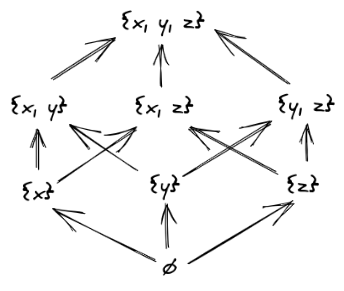
\includegraphics[scale=.4]{pics/pic_0.png}
                    
                    \begin{tikzpicture}
                        \node (a) at (0, 0) {$\set{x, y, z}$};
                        
                        \node (b0) at (-2, -1) {$\set{x, y}$};
                        \node (b1) at (0, -1) {$\set{x, z}$};
                        \node (b2) at (2, -1) {$\set{y, z}$};
                        
                        \node (c0) at (-2, -2) {$\set{x}$};
                        \node (c1) at (0, -2) {$\set{y}$};
                        \node (c2) at (2, -2) {$\set{z}$};
                        
                        \node (d) at (0, -3) {$\varnothing$};
                        
                        \draw[->] (d) -- (c0);
                        \draw[->] (d) -- (c1);
                        \draw[->] (d) -- (c2);
                        
                        \draw[->] (c0) -- (b0);
                        \draw[->] (c0) -- (b1);
                        
                        \draw[->] (c1) -- (b0);
                        \draw[->] (c1) -- (b2);
                        
                        \draw[->] (c2) -- (b1);
                        \draw[->] (c2) -- (b2);
                        
                        \draw[->] (b0) -- (a);
                        \draw[->] (b1) -- (a);
                        \draw[->] (b2) -- (a);
                    \end{tikzpicture}
                \end{center}
            \end{indt}
            
            \vspace{6pt}
            
            \begin{indt}{\subsubsection{Définition (ordre total)}}
                Soit $(E, \ \le)$ un ensemble ordonné.
                
                La relation d'ordre $\le$ est totale si, et seulement si :
                    \[ \forall x, y \in E,\ x \le y\ \text{ou}\ y \le x \]
                
                On dit alors que $E$ est totalement ordonné.
            \end{indt}
            
            \vspace{6pt}
            
            \begin{indt}{\subsubsection{Exemple}}
                $\bullet$ $\le$ sur $\N,\ \Z, \ \R$ est total.
                
                \vspace{6pt}
                
                $\bullet$ $(\mathcal P(E),\ \subseteq)$ n'est pas toujours total (s'il y a au moins 2 éléments $x, y \in E$, $\{x\}$ et $\{y\}$ ne sont pas comparables).
                
                \vspace{6pt}
                
                $\bullet$ $(\N,\ |)$ n'est pas total : $2 \nmid 3$ et $3 \nmid 2$.
            \end{indt}
            
            \vspace{6pt}
            
            \begin{indt}{\subsubsection{Définition (élément minimal / mininum)}}
                Soit $(E,\ \le)$ un ensemble ordonné et $P \in \mathcal P(E)$.
                
                $\bullet$ Un élément \textit{minimal} de $P$ est un élément $x \in P$ tel que :
                    \[ \forall y \in P,\ y \le x \Rightarrow y = x \]
                
                $\bullet$ Un \textit{minimum} pour $P$ est un élément $x \in P$ tel que :
                    \[ \forall y \in P,\ x \le y \]
            \end{indt}
            
            \vspace{6pt}
            
            \begin{indt}{\subsubsection{Remarque}}
                Le minimum, s'il existe, est unique et est minimal.
                
                Si l'ordre est total, être minimal est équivalent à être minimum.
                
                Il peut y avoir plusieurs éléments minimaux. Par exemple, avec $\{2, 3, 6, 9\}$ pour $(\N,\ |)$, 2 et 3 sont minimaux.
            \end{indt}
        \end{indt}
        
        \vspace{12pt}
        
        \begin{indt}{\subsection{Ordres et inductions bien fondés}}
            \begin{indt}{\subsubsection{Définition (ordre bien fondé)}}
                Soit $(E,\ \le)$ un ensemble ordonné.
                
                On dit que $(E,\ \le)$ est un \textit{ensemble bien fondé}, ou que $\le$ est un \textit{ordre bien fondé} si, et seulement si :
                    \[ \forall P \in \mathcal P(E) \setminus \{ \varnothing \},\ P\ \text{admet un élément minimal} \]
            \end{indt}
            
            \vspace{6pt}
            
            \begin{indt}{\subsubsection{Exemple}}
                $(\N,\ \le)$ et $(\N, \ |)$ sont bien fondés.
                
                $(\Z,\ \le)$ n'est pas bien fondé car $\Z$ n'admet pas d'élémement minimal.
                
                $(\Z,\ |)$ n'est pas ordonné.
                
                \vspace{6pt}
                
                \boxed{\rm Exo} Définir un ordre bien fondé sur $\Z$.
            \end{indt}
            
            \vspace{6pt}
            
            \begin{indt}{\subsubsection{Proposition}}
                Soit $(E,\ \le)$ un ensemble ordonné.
                
                \[ \le\ \text{bien fondé} \ssi \nexists (u_n)_{n \in \N} \subset E\ |\ \forall n \in \N,\ u_{n + 1} < u_n \]
                
                %\vspace{6pt}
                \newpage
                
                $\square$ Démonstration :
                
                $\Rightarrow$
                
                Supposons $\exists (u_n)_{n \in \N} \in E^\N$ strictement décroissante.
                
                On note $P = \{u_n\ |\ n \in \N\} \neq \varnothing$.
                
                Comme l'ordre est bien fondé, $P$ admet un élément minimal $u_n$ pour $n \in \N$.
                
                Or $u_{n + 1} \in P$ et $u_{n + 1} < u_n$, \textit{i.e} $u_{n + 1} \neq u_n$ et $u_{n + 1} \le u_n$.
                
                Or $u_{n + 1} \le u_n \Rightarrow u_{n + 1} = u_n$ par minimalité de $u_n$ : contradiction.
                
                \vspace{6pt}
                
                $\Leftarrow$
                
                Soit $P \in \mathcal P(E) \setminus \{\varnothing\}$.
                
                $\exists u_0 \in P$.
                
                Si $u_0$ est minimal, c'est fini. Sinon, $\exists u_1 \in P\ |\ u_1 < u_0$ et on recommence.
                
                On construit ainsi une suite strictement décroissante d'éléments de $P$, qui est nécessairement finie par hypothèse sur $(E, \le)$.
                
                Donc $\exists n \in \N\ |\ u_n$ est minimal dans $P$
                $\blacksquare$
            \end{indt}
            
            \vspace{6pt}
            
            \begin{indt}{\subsubsection{Remarque}}
                On peut généraliser la notion de variant en considérant une quantité strictement décroissante dans un ensemble bien fondé.
            \end{indt}
            
            \vspace{6pt}
            
            \begin{indt}{\subsubsection{Ordre produit}}
                $\bullet$ Définition : Soient $(E_1,\ \le_1)$ et $(E_2,\ \le_2)$ des ensembles ordonnés.
                
                On définit l'ordre produit $\le$ sur $E_1 \times E_2$ par :
                    \[ \forall ((x_1, y_1), (x_2, y_2)) \in {E_1}^2 \times {E_2}^2,\quad (x_1, x_2) \le (y_1, y_2) \ssi \eqsys{x_1 \le_1 y_1}{x_2 \le_2 y_2} \]
                
                \vspace{6pt}
                
                $\bullet$ Proposition : le produit de deux ordres bien fondés est bien fondé.
                
                $\bullet$ Remarque : Le produit de deux ordres n'est pas forcément total même si les deux ordres le sont.
            \end{indt}
            
            \vspace{6pt}
            
            \begin{indt}{\subsubsection{Ordre lexicographique}}
                $\bullet$ Définition : Soit $(E_1,\ \le_1)$ et $(E_2, \ \le_2)$ deux ensembles ordonnés.
                
                On définit l'ordre lexicographique sur $E_1 \times E_2$ par :
                
                \vspace{6pt}
                    
                    $
                        \forall ((x_1, y_1), (x_2, y_2)) \in {E_1}^2 \times {E_2}^2,\quad
                        (x_1, x_2) \le (y_1, y_2) \ssi x_1 <_1 y_1 \ \text{ou}\ \eqsys{x_1 = y_1}{x_2 \le_2 y_2}
                    $
                
                \vspace{12pt}
                
                $\bullet$ Proposition : L'ordre lexicographique issu de deux ordres bien fondés (resp. totaux) est bien fondé (resp. total).
                
                \vspace{6pt}
                
                $\bullet$ Remarque : On peut généraliser l'ordre lexicographique aux $n$-uplets ou aux suites finies (pas nécessairement de même longueur) dans un ensemble ordonné (ex : l'ordre du dictionnaire).
                
                \boxed{\rm Exo} : utiliser un ordre lexicographique pour prouver la terminaison de l'algorithme d'Euclide (PGCD)
            \end{indt}
            
            \vspace{6pt}
            
            \begin{indt}{\subsubsection{Théorème (principe d'induction bien fondée)}}
                On parle aussi d'induction noethérienne en l'honneur d'Emmy Noether (1882 - 1935).
                
                \vspace{6pt}
                
                Soit $(E,\ \le)$ un ensemble bien fondé et $P$ un prédicat sur cet ensemble
                ($P : E \longrightarrow \mathrm{bool}$). On a :
                    \[ (\forall x \in E,\ P(x)) \ssi (\forall x \in E,\ (\forall y \in E,\ y < x \Rightarrow P(y)) \Rightarrow P(x)) \]
                
                $\square$ Démonstration :
                
                $\Rightarrow$ évident.
                
                $\Leftarrow$ Supposons $\exists x \in E\ |\ P(x)$ soit faux.
                
                On note $Q = \{ y \in E\ |\ P(y)\ \text{faux} \}$.
                
                $x \in Q$, donc $Q \neq \varnothing$.
                
                $(E,\ \le)$ est bien fondé, donc $Q$ admet un élément minimal $x_0$.
                
                On sait que $(\forall y \in E,\ y < x_0 \Rightarrow P(y)) \Rightarrow P(x_0)$
                
                Montrons que $\forall y \in E,\ y < x_0 \Rightarrow P(y)$, ce qui conclut car $P(x_0)$ est faux ($x_0 \in Q$).
                
                Soit $y \in E\ |\ y < x_0$.
                
                On ne peut pas avoir $P(y)$ faux, car sinon $y \in Q$ et $y < x_0$ minimal dans $Q$.
                
                Donc $P(y)$ vrai $\blacksquare$
            \end{indt}
            
            \vspace{6pt}
            
            \begin{indt}{\subsubsection{Remarque}}
                \label{1.2.8}
                \begin{indt}{$\bullet$ Le principe d'induction bien fondée donne une méthode de démonstration d'un prédicat $P$ :}
                    $-$ Initialisation : $\forall x \in E$ minimal, on démontre $P(x)$
                    
                    $-$ Hérédité : $\forall x \in E\ |\ \forall y \in E,\ y < x \Rightarrow P(y)$, on démontre $P(x)$.
                \end{indt}
                
                \vspace{6pt}
                
                $\bullet$ Le principe d'induction bien fondée généralise le principe de récurrence forte (sur $(\N, \ \le)$) ;
                
                \vspace{6pt}
                
                $\bullet$ Le principe d'induction bien fondée généralise aussi le principe de récurrence (si l'on considère des relations bien fondées qui ne sont pas forcément des ordres : $(\N,\ <)$ où $x < y \ssi y = x + 1$) ;
                
                \vspace{6pt}
                
                $\bullet$ Le principe d'induction bien fondée généralise également un autre principe d'induction lié à la défintion d'ensembles à la manière des types sommes en OCaml (et donc aussi du filtrage par motif).
            \end{indt}
        \end{indt}
        
    \end{indt}
    
    \vspace{12pt}
    
    \begin{indt}{\section{Ensembles inductifs, induction structurelle}}
        
        \begin{indt}{\subsection{Définition par induction}}
            \begin{indt}{\subsubsection{Définition (système de règles d'inférence)}}
                Un \textit{système de règles d'inférences} est donné par un ensemble d'assertions (propriétés) et de règles pour démontrer ces assertions (on parle de règles d'inférence).
                Une règle d'inférence est donnée par un ensemble de $n \in \N$ prémisses (hypothèses de la règle) et par une assertion qu'on appelle la conclusion. On note une telle règle :
                    \[ \dfrac{\text{prémisse}_1\ \text{prémisse}_2\ \ldots\ \text{prémisse}_n}{\text{conclusion}} \]
                Si $n = 0$, on parle d'axiome.
            \end{indt}
            
            \vspace{12pt}
            
            \begin{indt}{\subsubsection{Exemple}}
                Avec l'assertion \simplecit{être un entier naturel}, on peut définir les règles :
                    \[
                        \dfrac{}{0\ \text{est un entier naturel}} (0)
                        \quad \text{et} \quad
                        \dfrac{n\ \text{est un entier naturel}}{S(n)\ \text{est un entier naturel}} (S)
                    \]
                
                Où $S(n)$ est le successeur de $n$.
            \end{indt}
            
            \vspace{12pt}
            
            \begin{indt}{\subsubsection{Définition (dérivation)}}
                \'Etant donné un système de règles d'inférences, une assertion est dite \textit{dérivable} si elle est la conclusion d'un axiome ou d'une règle dont les prémisses sont dérivables.
                
                On appelle (arbre de) dérivation l'ensemble des règles utilisées pour dériver une assertion.
            \end{indt}
            
            \vspace{12pt}
            
            \begin{indt}{\subsubsection{Exemple}}
                On ajoute un opérateur $+$ et la règle :
                    \[ \dfrac{n\ \text{est un entier naturel}\ m\ \text{est un entier naturel}}{n + m\ \text{est un entier naturel}} (+) \]
                
                On peut alors dériver l'assertion $S(S(0)) + S(0)$ est un entier naturel :
                    \[
                        \dfrac{
                            \dfrac{
                                \dfrac{
                                    \dfrac{}{0\ \text{est un entier naturel}} (0)
                                }
                                {
                                    S(0)\ \text{est un entier naturel}
                                } (S)
                            }
                            {
                                S(S(0))\ \text{est un entier naturel}} (S)\
                                \dfrac{
                                    \dfrac{}{0\ \text{est un entier naturel}} (0)
                                }
                                {
                                    S(0)\ \text{est un entier naturel}
                                } (S)
                        }
                        {
                            S(S(0)) + S(0)\ \text{est un entier naturel}
                        }
                            (+)
                    \]
                
                %Try package \texttt{mathpartir}
            \end{indt}
            
            \vspace{12pt}
            
            \begin{indt}{\subsubsection{Définition (ensemble inductif)}}
                Un \textit{ensemble inductif}, ou ensemble défini par induction, est le plus petit ensemble (au sens de l'inclusion) engendré par un système de règles d'inférence (avec l'assertion \simplecit{appartient à cet ensemble}).
            \end{indt}
            
            \vspace{12pt}
            
            \begin{indt}{\subsubsection{Exemple}}
                On définit inductivement l'ensemble \textsl{Expr} des expressions arithmétiques sur les entiers naturels par :
                    \[ \begin{array}{cc}
                        \dfrac{n \in \N}{n \in \text{\sl Expr}} (\text{\sl nat})
                        & \dfrac{e_1 \in \text{\sl Expr}\ e_2 \in \text{\sl Expr}}{e_1 + e_2 \in \text{\sl Expr}} (+)
                        \\\\
                        \dfrac{e_1 \in \text{\sl Expr}\ e_2 \in \text{\sl Expr}}{e_1 - e_2 \in \text{\sl Expr}} (-)
                        & \dfrac{e_1 \in \text{\sl Expr}\ e_2 \in \text{\sl Expr}}{e_1 * e_2 \in \text{\sl Expr}} (*)
                    \end{array} \]
            \end{indt}
            
            \vspace{12pt}
            
            \begin{indt}{\subsubsection{Remarque}}
                On procède de manière analogue à la définition d'un type somme récursif en OCaml en associant une règle à chaque constructeur du type : si le constructeur n'a pas d'argument, alors il correspond à un axiome, sinon, la règle qui lui correspond à pour prémisses l'appartenance des arguments à leurs types respectifs.
                
                \begin{lstlisting}[language=Caml, xleftmargin=80pt]
type expr =
    | Nat of nat
    | Plus of expr*expr
    | Minus of expr*expr
    | Mult of expr*expr
and nat =
    | Zero
    | S of nat
                \end{lstlisting}
            \end{indt}
        \end{indt}
            
        \vspace{12pt}
        
        \begin{indt}{\subsection{Preuves par induction}}
            \begin{indt}{\subsubsection{Définition (ordre induit par une définition inductive)}}
                Soit $E$ un ensemble inductif. On peut définir un ordre sur $E$ par :
                
                $\forall x, y \in E,\ x \le y \ssi$l'assertion $x \in E$ apparait dans une dérivation de taille minimale (en termes du nombre de règles utilisées) de l'assertion $y \in E$.
                
                \vspace{12pt}
                %\newpage
                
                $\square$ Démonstration :
                
                $-$ Réflexivité : $\forall x \in E,\ x \le x$ car $x \in E$ est la conclusion de la dérivation ;
                
                \vspace{6pt}
                
                $-$ Transitivité : Soient
                $
                    x, y, z \in E\
                    \left| \!
                    \begin{array}{l}
                        x \le y
                        \\
                        y \le z
                    \end{array}
                    \right.
                $
                
                L'assertion $y \in E$ apparaît dans une dérivation minimale de $z \in E$. Dans cette dérivation on utilise bien une dérivation minimale de $y \in E$ (sinon on pourrait réduire la taille de la dérivation de $z \in E$). Donc l'assertion $x \in E$ y apparait. Donc $x \le z$ ;
                
                \vspace{6pt}
                
                $-$ Antisymétrie : Soient
                $
                    x, y \in E\
                    \left| \!
                    \begin{array}{l}
                        x \le y
                        \\
                        y \le x
                    \end{array}
                    \right.
                $
                
                Si $x \neq y$, dans une dérivation minimale de $x \in E$, on trouve une dérivation minimale de $y \in E$, qui elle-même contient une dérivation de $x \in E$, nécessairement strictement plus petite, ce qui est absurde.
                $\blacksquare$
            \end{indt}
            
            \vspace{12pt}
            
            \begin{indt}{\subsubsection{Exemple}}
                L'ordre induit sur les entiers naturels donne l'ordre usuel.
                
                L'ordre induit sur les expressions arithmétiques est la propriété d'être une sous-expression (ex : $S(0) + 0 \le (S(0) + 0) * S(S(0))$)
            \end{indt}
            
            \vspace{12pt}
            
            \begin{indt}{\subsubsection{Proposition (admise)}}
                L'ordre induit sur les ensembles inductifs est bien fondé.
            \end{indt}
            
            \vspace{12pt}
            
            \begin{indt}{\subsubsection{Corollaire}}
                On peut utiliser le principe d'induction bien fondée sur les ensembles inductifs.
            \end{indt}
            
            \vspace{12pt}
            
            \begin{indt}{\subsubsection{Remarque}}
                Soit $E$ un ensemble inductif.
                
                On peut, comme dans la remarque \ref{1.2.8}, se passer de l'ordre induit pour lui préférer la relation bien fondée $x < y \ssi x \in E$ est une prémisse de la dernière règle d'une dérivation de $y \in E$.
                
                On obtient alors le principe d'\textit{induction structurelle} que l'on peut écrire aussi :
                
                Soit $P$ in prédicat sur $E$.
                Si pour toute règle d'inférence de la forme
                    \[ \dfrac{x_1 \in E\ \ldots\ x_n \in E}{C(x_1\ \ldots\ x_n) \in E} \]
                on a la propriété
                    \[ \forall (x_k)_{k \in \nset 1 n} \subset E,\ \forall k \in \nset 1 n,\ P(x_k) \Rightarrow P(C(x_1\ \ldots\ x_n)) \]
                alors $\forall x \in E,\ P(x)$.
            \end{indt}
            
            \vspace{12pt}
            
            \begin{indt}{\subsubsection{Exemple}}
                On retrouve le principe de récurrence sur les entiers naturels.
                
                \vspace{6pt}
                
                On démontre par induction structurelle que la valeur associée à toute expression arithmétique ne faisant pas intervenir le symbole $-$ est positive :
                
                $-$ Règle (\textsl{nat}) : si $n \in \N$, alors $n \ge 0$ (par induction structurelle sur les entiers naturels)
                
                $-$ Règle $(+) / (*)$ : si $e_1, e_2 \in $ \textsl{Expr} ne font pas intervenir le symbole $(-)$, alors par induction $e_1 \ge 0$ et $e_2 \ge 0$
                
                Donc $e_1 + e_2 \ge 0$  et $e_1 * e_2 \ge 0$.
            \end{indt}
        \end{indt}
            
        \vspace{12pt}
        
        \begin{indt}{\subsection{Justification des définitions par induction (H.P)}}
            \begin{indt}{\subsubsection{Définition (treillis complet)}}
                Soit $(E,\ \le)$ un ensemble ordoné.
                
                $(E, \ \le)$ est un \textit{treillis complet} si, et seulement si :
                    \[
                        \forall A \in \mathcal P(E),\
                        \eqsys
                            {A\ \text{admet un plus grand minorant}\ \wedge A}
                            {A\ \text{admet un plus petit majorant}\ \vee A}
                    \]
                
                Rappel :
                
                $-$ $m$ est un majorant pour $A$ $\ssi \forall a \in A,\ a \le m$
                
                $-$ $m = \vee A \ssi m$ est un majorant et $\forall m'$ majorant de $A, m \le m'$
            \end{indt}
            
            \vspace{12pt}
            
            \begin{indt}{\subsubsection{Proposition}}
                Soit $E$ un ensemble.
                
                Alors $(\mathcal P(E),\ \subseteq)$ est un treillis comlet.
                
                \vspace{12pt}
                
                $\square$ Démonstration :
                
                Soit $A \in \mathcal P(\mathcal P(E))$. On définit
                    \[
                        \eqsys
                            {\displaystyle \cap A = \bigcap_{P \in A} P \quad (E\ \text{si}\ A \neq \varnothing)}
                            {\displaystyle \cup A = \bigcup_{P \in A} P \quad (\varnothing\ \text{si}\ A \neq \varnothing)}
                    \]
                \boxed{\rm Exo} : $\cap A = \wedge A$ et $\cup A = \vee A$
            \end{indt}
            
            \vspace{12pt}
            
            \begin{indt}{\subsubsection{Théorème (Knaster - Tarski)}}
                Soit $(E, \ \le)$ un treillis complet et $f : E \longrightarrow E$ croissante.
                
                On définit l'ensemble des pré-points fixes de $f$ par
                    \[ P_f = \set{x \in E,\ |\ f(x) \le x} \]
                
                Alors $\wedge P_f$ est un point fixe de $f$ (le plus petit)
                
                \vspace{12pt}
                
                $\square$
                Soit $x \in P_f$.
                
                Alors par définition, $\wedge P_f \le x$, donc par croissance de $f$, $f(\wedge P_f) \le f(x) \le x$.
                
                Donc $f(\wedge P_f)$ est un minorant de $P_f$.
                
                Donc par définition, $f(\wedge P_f) \le \wedge P_f$ donc par croissance, $f(f(\wedge P_f)) \le f(\wedge P_f)$
                
                donc $f(\wedge P_f) \in P_f$, donc par définition, $\wedge P_f \le f(\wedge P_f)$
                
                donc par antisymétrie, $\boxed{f(\wedge P_f) = \wedge P_f}$
                $\blacksquare$
            \end{indt}
            
            \vspace{12pt}
            
            \begin{indt}{\subsubsection{Application (définition d'ensemble inductif)}}
                \'Etant donné des ensembles prédéfinis $B_1,\ \ldots,\ B_t$, on définit par induction un ensemble à l'aide de constructeurs $C_1,\ \ldots,\ C_k$ où $\forall i \in \nset 1 k,\ C_i$ est associé à un tuple de type d'arguments ${a_i}^1,\ \ldots\ {a_i}^{n_i}$ où $\forall j \in \nset 1 {n_i}$,
                    \[ {a_i}^j = \eqsys{B_m\ \text{pour un certain $m$}}{\text{rec (cas d'induction)}} \]
                
                On définit alors
                
                    \[ \displaystyle f_{C_1\ \ldots\ C_k}(S) = \bigcup_{i \in \nset 1 k} \set{C_i(u_1\ \ldots u_{n_i}),\ \forall j \in \nset 1 {n_i}, \eqsys{u_j \in B_m\ \text{si $a_i^j = B_m$}}{u_j \in S\ \text{si $a_i^j =$ rec}}} \]
                
                On admet que $f_{C_1\ \ldots C_k}$ est croissante sur le treillis complet des parites.
                
                Le théorème de Knaster-Tasrski assure l'existence du plus petit ensemble stable par application des constructeurs, \textit{i.e} l'ensemble inductif défini par les $C_i$.
            \end{indt}
            
            \vspace{12pt}
            
            \begin{indt}{\subsubsection{Remarque}}
                On pourrait de même utiliser les théorème de Knaster-Tarski pour justifier le principe d'induction structurelle, ou pour justifier la définition par induction de fonctions sur un ensemble inductif.
                
                Ceci permet donc le filtrage par motif.
                
                Finalement, on a défini inductivement la notion de dérivation, on peut donc faire des preuves par induction structurelle sur les dérivations.
            \end{indt}
        \end{indt}
        
    \end{indt}

    

    
    
\end{document}
%--------------------------------------------End
